\subsection{Set Theory}
\hrulefill\\

\subsubsection*{Definitions}
\begin{align*}
    A \subseteq B &\iff \forall x \in A \implies x \in B\\
    A \nsubseteq B &\iff \exists x \in A \implies x \neq B\\
\end{align*}

A is a \textbf{proper subset} of B ($A \subset B$) if and only if:
\begin{itemize}
    \item $A \subseteq B$ and
    \item $\exists x$ such that $x \in B$ and $x \notin A$
\end{itemize}

\paragraph*{Example}
Let 
\begin{align*}
    A &= \{m \in \mathbb{Z} | \exists r \in \mathbb{Z} \ni m = 6r + 12\}\\
    B &= \{n \in \mathbb{Z} | \exists s \in \mathbb{Z} \ni n = 3s\}\\
    \\
    A \subseteq B?:\\
    &6r + 12 = 6(r + 2) \implies A = \{m \in \mathbb{Z} | \exists t \in \mathbb{Z} \ni m = 6t\}\\
    &m = 6n \implies m = 3(2n)\\
    \therefore \quad & A \subseteq B\\
\end{align*}

\subsubsection*{Set Equivalence}
\paragraph*{Definition}
Given sets A and B:
\begin{equation}
    A = B \iff A \subseteq B \land B \subseteq A
\end{equation}

\paragraph*{Example}
Let
\begin{align*}
    R &= \{x \in \mathbb{Z} : 2|x\}\\
    T &= \{x \in \mathbb{Z} : 6|x\}\\
    \\
    R \subseteq T &\equiv \text{False}\\
    & Let x \in R and x = 2(1) = 2, \text{ but } 2 \neq 6k \forall k \in \mathbb{Z}\\
    \implies \quad & x \notin T\\
    \therefore \quad & R \nsubseteq T\\
    \\
    T \subseteq R &\equiv \text{True}\\
    \therefore \quad & R \neq T\\
    & Let x \in T\\
    \implies \quad & \exists k \in \mathbb{Z} \ni x = 6k \implies x = 2(3k)\\
    \implies \quad & 3k \in \mathbb{Z} \implies 2 | x \implies x \in R\\
    \therefore \quad & T \subseteq{R}
\end{align*}

\begin{center}
    \includegraphics*[width=\textwidth]{venn-diagrams.png}\\
    \includegraphics*[width=\textwidth]{set-operations.png}
\end{center}

\paragraph*{Example}
Let 
\begin{align*}
    U &= \{1, 2, 3, 4, 5, 6, 7\}\\
    A &= \{1, 3, 5, 7\}\\
    B &= \{4, 5, 6, 7\}\\
    \\
    A \cup B &= \{1, 3, 4, 5, 6, 7\}\\
    A \cap B &= \{5, 7\}\\
    B - A &= \{4, 6\}\\
    A^c &= \{2, 4, 6\}
\end{align*}

\subsubsection*{Interval Notation}
\includegraphics*[width=\textwidth]{interval-notation.png}

\paragraph*{Example}
Let $U = \mathbb{R}$,$A = (-1, 0]$ and $B = [0, 1)$
\begin{align*}
    A \cup B &= \{-1, 1\}\\
    A \cap B &= \{0\}\\
    B - A &= (0, 1)\\
    A^c &= (- \infty, 1] \cup (0, \infty)
\end{align*}

\subsubsection*{Disjoint Sets}
\paragraph*{Definition}
\begin{center}
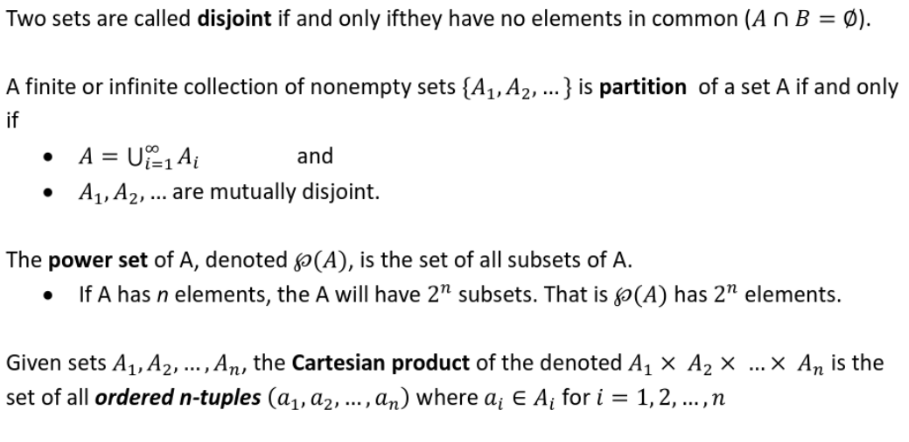
\includegraphics[width=\textwidth]{disjoint-sets.png}    
\end{center}


\paragraph*{Example}
Find $\mathcal{P}(A)$ if $A = \{1,2\}$
\begin{align*}
    \mathcal{P}(A) = \{\varnothing, 1, 2, (1,2)\}
\end{align*}